\documentclass{ximera}
\input{../preamble.tex}

\title{Exercises} \license{CC BY-NC-SA 4.0}

\begin{document}

\begin{abstract}
\end{abstract}
\maketitle

\begin{onlineOnly}
\section*{Exercises}
\end{onlineOnly}


\begin{problem}\label{exer:6.3.1}
Find the current in the
$RLC$ circuit, assuming that $E(t)=0$ for $t>0$.  $R=3$ ohms;  \, $L=.1$ henrys;  \, $C=.01$ farads;   $Q_0=0$
coulombs;  \,$I_0=2$ amperes.
\end{problem}

\begin{problem}\label{exer:6.3.2}
Find the current in the
$RLC$ circuit, assuming that $E(t)=0$ for $t>0$.  $R=2$ ohms;  \, $L=.05$ henrys;  \, $C=.01$ farads';  $Q_0=2$
coulombs;  \,$I_0=-2$ amperes.

\begin{solution}
    $\frac{1}{20}Q''+2Q'+100Q=0$;\, $Q''+40Q'+2000Q=0$;\,
$r^2+40r+2000=(r+20)^2+1600=0$;\,
$r=-20\pm40i$;\,
$Q=e^{-20t}(2\cos40t+c_2\sin40t)$ (since $Q_0=2$);\,
$I=Q'=e^{-20t}\left((40c_2-40)\cos40t-(20c_2+80)\sin40t\right)$;\,
$I_0=2\Rightarrow 40c_2-40=2\Rightarrow c_2=\frac{21}{20}$,
so $20c_2+80=101$;\,
$I=e^{-20t}(2\cos40t-101\sin40t)$.
\end{solution}
\end{problem}

\begin{problem}\label{exer:6.3.3}
Find the current in the
$RLC$ circuit, assuming that $E(t)=0$ for $t>0$.  $R=2$ ohms;  \, $L=.1$ henrys;  \, $C=.01$ farads;   $Q_0=2$
coulombs;  \,$I_0=0$ amperes.
\end{problem}

\begin{problem}\label{exer:6.3.4}
Find the current in the
$RLC$ circuit, assuming that $E(t)=0$ for $t>0$.  $R=6$ ohms;  \, $L=.1$ henrys;  \, $C=.004$ farads';  $Q_0=3$
coulombs;  \,$I_0=-10$ amperes.

\begin{solution}
    $\frac{1}{10}Q''+6Q'+250Q=0$;\, $Q''+60Q'+2500Q=0$;\,
$r^2+60r+2500=(r+30)^2+1600=0$;\,
$r=-30\pm40i$;\,
$Q=e^{-30t}(3\cos40t+c_2\sin40t)$ (since $Q_0=3$);\,
$I=Q'=e^{-30t}\left((40c_2-90)\cos40t-(30c_2+120)\sin40t\right)$;\,
$I_0=-10\Rightarrow 40c_2-90=-10\Rightarrow c_2=2$,
so $-30c_2-120=-180$;\,
$I=-10e^{-30t}(\cos40t+18\sin40t)$.
\end{solution}
\end{problem}

\begin{problem}\label{exer:6.3.5}
Find the current in the
$RLC$ circuit, assuming that $E(t)=0$ for $t>0$.  $R=4$ ohms;  \, $L=.05$ henrys;  \, $C=.008$ farads;   $Q_0=-1$
coulombs;  \,$I_0=2$ amperes.
\end{problem}

\begin{problem}\label{exer:6.3.6}
Find the steady
state current in the circuit described by the  equation.
$\frac{1}{10}Q''+3Q'+100Q=5\cos10t-5\sin10t$

\begin{solution}
    $Q_p=A\cos10t+B\sin10t$;
$Q_p'=10B\cos10t-10A\sin10t$;
$Q_p''=-100A\cos10t-100B\sin10t$;
$\frac{1}{10}Q_p''+3Q_p'+100Q_9=
(90A+30B)\cos10t-(30A-90B)\sin10t=5\cos10t-5\sin10t$,
so $90A+30B=5$, $-30A+90B=-5$. Therefore, $A=1/15$, $B=-1/30$,
$Q_p=\frac{\cos10t}{15}-\frac{\sin10t}{30}$, and
$I_p=-\frac{1}{3}(\cos10t+2\sin10t)$.
\end{solution}
\end{problem}

\begin{problem}\label{exer:6.3.7}
Find the steady
state current in the circuit described by the  equation.
$\frac{1}{20}Q''+2Q'+100Q=10\cos25t-5\sin25t$
\end{problem}

\begin{problem}\label{exer:6.3.8}
Find the steady
state current in the circuit described by the  equation.
$\frac{1}{10}Q''+2Q'+100Q=3\cos50t-6\sin50t$

\begin{solution}
    $Q_p=A\cos 50t+B\sin 50t$;
$Q_p'=50B\cos 50t-50A\sin 50t$;
$Q_p''=-2500A\cos 50t-2500B\sin 50t$;
$\frac{1}{10}Q_p''+2Q_p'+100Q_p
(-150A+100B)\cos 50t-(100A+150B)\sin 50t=3\cos50t-6\sin50t$,
so $-150A+100B=3$, $-100A+150B=-6$. Therefore,$A=3/650$,
$B=12/325$, $Q_p=\frac{3}{650}(\cos50t+8\sin50t)$, and
$I_p= \frac{3}{13}(8\cos50t-\sin50t)$.
\end{solution}
\end{problem}

\begin{problem}\label{exer:6.3.9}
Find the steady
state current in the circuit described by the  equation.
$\frac{1}{10}Q''+6Q'+250Q=10\cos100t+30\sin100t$
\end{problem}

\begin{problem}\label{exer:6.3.10}
Find the steady
state current in the circuit described by the  equation.
$\frac{1}{20}Q''+4Q'+125Q=15\cos30t-30\sin30t$

\begin{solution}
    $Q_p=A\cos 30t+B\sin 30t$;
$Q_p'=30B\cos 30t-30A\sin 30t$;
$Q_p''=-900A\cos 30t-900B\sin 30t$;
$\frac{1}{20}Q_p''+4Q_p'+125Q_p=
(80A+120B)\cos 30t-(120A-80B)\sin 30t=15\cos30t-30\sin30t$, so
$80A+120B=15$, $-120A+80B=-30$,
$A=3/13$, $B=-3/104$,
$Q_p=
\frac{3}{104}(8\cos 30t-\sin 30t)$, and
$I_p=-\frac{45}{52}(\cos30t+8\sin30t)$.
\end{solution}
\end{problem}

\begin{problem}\label{exer:6.3.11}  Consider the circuit below.

\begin{center}
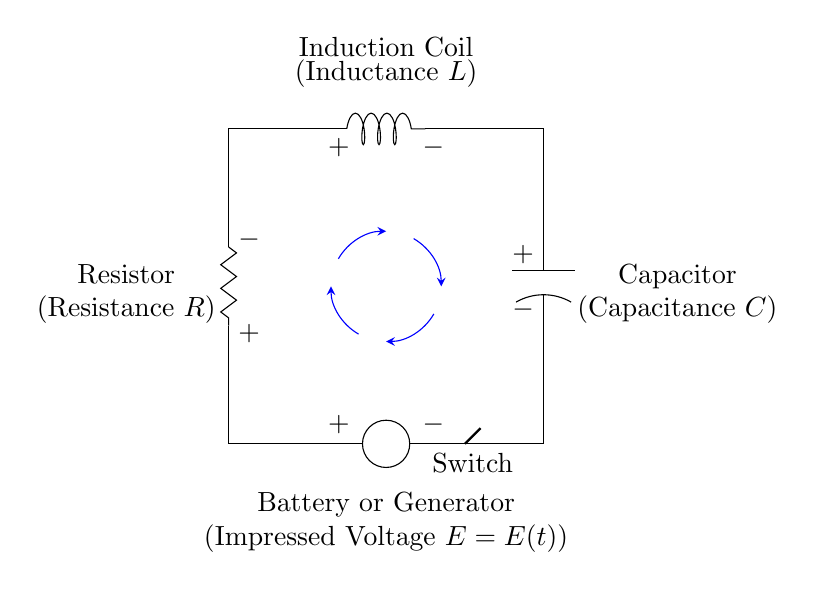
\begin{tikzpicture}[scale=1]

% Box
\draw[black] (-2,0.5) -- (-2,2) -- (-0.5,2);
\draw[black] (0.5,2) -- (2,2) -- (2,0.2);
\draw[black] (2,-0.1) -- (2,-2) -- (0.5,-2);
\draw[black] (0.5,-2) -- (-2,-2) -- (-2,-0.5);

% Inductor (coil) on top
\draw[black,decorate,decoration={coil,aspect=0.3,segment length=2mm,amplitude=2mm}] 
      (-0.5,2) -- (0.5,2);

% Resistor (zigzag) on left
\draw[black,decorate,decoration={zigzag,segment length=3mm,amplitude=1mm}] 
      (-2,0.5) -- (-2,-0.5);

% Capacitor on right
\draw[black] (1.6,0.2) -- (2.4,0.2);
\draw[black](2.35,-0.2) arc[start angle=60, end angle=120, radius=0.7];
% Switch (bottom)
\draw[black, fill=white] (0,-2) circle(0.3); 
\draw[black,thick] (1,-2) -- (1.2,-1.8);

% Arrows (current direction)
\foreach \angle in {60,150,240,330} {
  \draw[-stealth,blue] (0,0) ++(\angle:0.7) arc[start angle=\angle, end angle=\angle-60, radius=0.7];
}

% Labels
\draw[black] (1.1,-2) node[below]{Switch};
\draw[black] (0,-2.5) node[below]{Battery or Generator};
\draw[black] (0,-2.9) node[below]{(Impressed Voltage $E=E(t)$)};
\draw[black] (-3.3,0.4) node[below]{Resistor};
\draw[black] (-3.3,0) node[below]{(Resistance $R$)};
\draw[black] (3.7,0.4) node[below]{Capacitor};
\draw[black] (3.7,0) node[below]{(Capacitance $C$)};
\draw[black] (0,2.4) node[above]{(Inductance $L$)};
\draw[black] (0,2.8) node[above]{Induction Coil};

\draw[black] (0.6,2) node[below]{$\boldsymbol{-}$};
\draw[black] (-0.6,2) node[below]{$\boldsymbol{+}$};

\draw[black] (-2,0.6) node[right]{$\boldsymbol{-}$};
\draw[black] (-2,-0.6) node[right]{$\boldsymbol{+}$};

\draw[black] (-0.6,-2) node[above]{$\boldsymbol{+}$};
\draw[black] (0.6,-2) node[above]{$\boldsymbol{-}$};

\draw[black] (2,0.4) node[left]{$\boldsymbol{+}$};
\draw[black] (2,-0.3) node[left]{$\boldsymbol{-}$};

\end{tikzpicture}
\end{center}

%\begin{image}
 % \includegraphics[height=1.5in]{fig060301.jpg}
%\end{image}

Show that if $E(t)=U\cos\omega t+V\sin\omega t$ where $U$
and $V$ are constants then the steady state current in
the $RLC$ circuit is
$$
I_p=\frac{\omega^2RE(t)+(1/C-L\omega^2)E'(t)}{\Delta},
$$
where
$$
\Delta=(1/C-L\omega^2)^2+R^2\omega^2.
$$
\end{problem}

\begin{problem}\label{exer:6.3.12}  Consider the circuit below.

\begin{center}
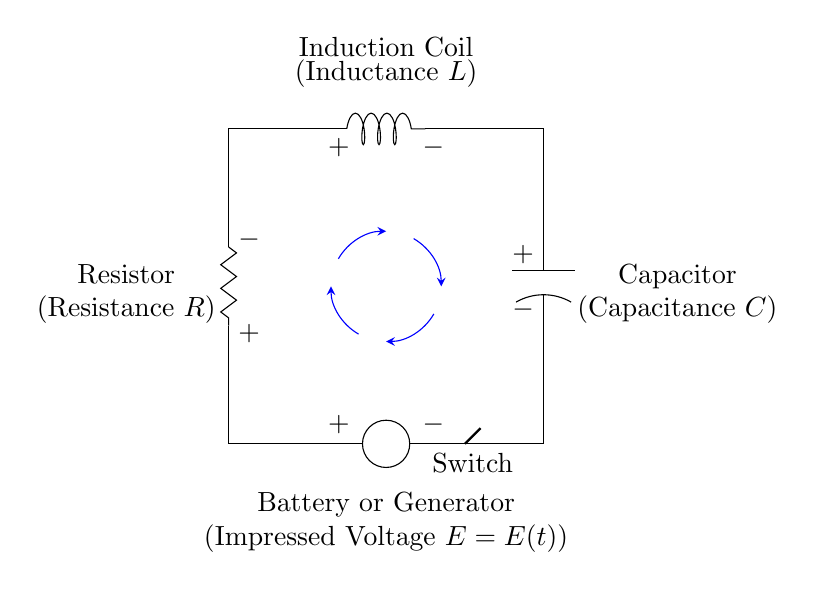
\begin{tikzpicture}[scale=1]

% Box
\draw[black] (-2,0.5) -- (-2,2) -- (-0.5,2);
\draw[black] (0.5,2) -- (2,2) -- (2,0.2);
\draw[black] (2,-0.1) -- (2,-2) -- (0.5,-2);
\draw[black] (0.5,-2) -- (-2,-2) -- (-2,-0.5);

% Inductor (coil) on top
\draw[black,decorate,decoration={coil,aspect=0.3,segment length=2mm,amplitude=2mm}] 
      (-0.5,2) -- (0.5,2);

% Resistor (zigzag) on left
\draw[black,decorate,decoration={zigzag,segment length=3mm,amplitude=1mm}] 
      (-2,0.5) -- (-2,-0.5);

% Capacitor on right
\draw[black] (1.6,0.2) -- (2.4,0.2);
\draw[black](2.35,-0.2) arc[start angle=60, end angle=120, radius=0.7];
% Switch (bottom)
\draw[black, fill=white] (0,-2) circle(0.3); 
\draw[black,thick] (1,-2) -- (1.2,-1.8);

% Arrows (current direction)
\foreach \angle in {60,150,240,330} {
  \draw[-stealth,blue] (0,0) ++(\angle:0.7) arc[start angle=\angle, end angle=\angle-60, radius=0.7];
}

% Labels
\draw[black] (1.1,-2) node[below]{Switch};
\draw[black] (0,-2.5) node[below]{Battery or Generator};
\draw[black] (0,-2.9) node[below]{(Impressed Voltage $E=E(t)$)};
\draw[black] (-3.3,0.4) node[below]{Resistor};
\draw[black] (-3.3,0) node[below]{(Resistance $R$)};
\draw[black] (3.7,0.4) node[below]{Capacitor};
\draw[black] (3.7,0) node[below]{(Capacitance $C$)};
\draw[black] (0,2.4) node[above]{(Inductance $L$)};
\draw[black] (0,2.8) node[above]{Induction Coil};

\draw[black] (0.6,2) node[below]{$\boldsymbol{-}$};
\draw[black] (-0.6,2) node[below]{$\boldsymbol{+}$};

\draw[black] (-2,0.6) node[right]{$\boldsymbol{-}$};
\draw[black] (-2,-0.6) node[right]{$\boldsymbol{+}$};

\draw[black] (-0.6,-2) node[above]{$\boldsymbol{+}$};
\draw[black] (0.6,-2) node[above]{$\boldsymbol{-}$};

\draw[black] (2,0.4) node[left]{$\boldsymbol{+}$};
\draw[black] (2,-0.3) node[left]{$\boldsymbol{-}$};

\end{tikzpicture}
\end{center}

%\begin{image}
 % \includegraphics[height=1.5in]{fig060301.jpg}
%\end{image}

Find the amplitude of the steady state current $I_p$ in the $RLC$
circuit if $E(t)=U\cos\omega
t+V\sin\omega t$, where $U$ and $V$ are constants. Then find the value
$\omega_0$ of $\omega$ maximizes the amplitude, and
 find the maximum amplitude.

 \begin{solution}
     Let $\sigma=\sigma(\omega)$ be the amplitude of $I_p$.
From the solution of  Exercise~6.3.11,
$Q_p=A\cos\omega t+B\cos\omega t$, where
$A=\frac{(1/C-L\omega^2)U-R\omega V}{\Delta}$,
$B=\frac{R\omega U+(1/C-L\omega^2)V}{\Delta}$,  and
$\Delta=(1/C-L\omega^2)^2+R^2\omega^2$. Since
$I_p=Q'_p=\omega(-A\sin\omega t+B\cos\omega t)$, it follows that
$\sigma^2(\omega)=\omega^2(A^2+B^2)=\frac{U^2+V^2}{\rho(\omega)}$,
with
$\rho(\omega)=\frac{\Delta}{\omega^2}=(1/C\omega-L\omega)^2+R^2$,
which attains it mininmum value $R^2$ when
$\omega=\omega_0=\frac{1}{\sqrt{LC}}$. The maximum amplitude of
$I_p$ is
$\sigma(\omega)=\frac{\sqrt{U^2+V^2}}{ R}$.
 \end{solution}
\end{problem}

\begin{problem}\label{exer:6.3.13} Plot the
amplitude of the steady state current against $\omega$. Estimate the
value of $\omega$ that maximizes the amplitude of the steady state
current, and estimate this maximum amplitude. 
\begin{hint}
    You can confirm
your results by doing Exercise~$\ref{exer:6.3.12}$.
\end{hint}
$\frac{1}{10}Q''+3Q'+100Q=U\cos\omega t+V\sin\omega t$
\end{problem}

\begin{problem}\label{exer:6.3.14} Plot the
amplitude of the steady state current against $\omega$. Estimate the
value of $\omega$ that maximizes the amplitude of the steady state
current, and estimate this maximum amplitude. 
\begin{hint}
    You can confirm
your results by doing Exercise~$\ref{exer:6.3.12}$.
\end{hint}
$\frac{1}{20}Q''+2Q'+100Q=U\cos\omega t+V\sin\omega t$
\end{problem}

\begin{problem}\label{exer:6.3.15} Plot the
amplitude of the steady state current against $\omega$. Estimate the
value of $\omega$ that maximizes the amplitude of the steady state
current, and estimate this maximum amplitude. 
\begin{hint}
    You can confirm
your results by doing Exercise~$\ref{exer:6.3.12}$.
\end{hint}
$\frac{1}{10}Q''+2Q'+100Q=U\cos\omega t+V\sin\omega t$
\end{problem}

\begin{problem}\label{exer:6.3.16} Plot the
amplitude of the steady state current against $\omega$. Estimate the
value of $\omega$ that maximizes the amplitude of the steady state
current, and estimate this maximum amplitude. 
\begin{hint}
    You can confirm
your results by doing Exercise~$\ref{exer:6.3.12}$.
\end{hint}
$\frac{1}{10}Q''+6Q'+250Q=U\cos\omega t+V\sin\omega t$
\end{problem}

\begin{problem}\label{exer:6.3.17}
Plot the
amplitude of the steady state current against $\omega$. Estimate the
value of $\omega$ that maximizes the amplitude of the steady state
current, and estimate this maximum amplitude. 
\begin{hint}
    You can confirm
your results by doing Exercise~$\ref{exer:6.3.12}$.
\end{hint}
$\frac{1}{20}Q''+4Q'+125Q=U\cos\omega t+V\sin\omega t$
\end{problem}

\end{document}